\documentclass{article}

\usepackage[utf8]{inputenc}
\usepackage[T1]{fontenc}
\usepackage[spanish]{babel}
\usepackage{times}
\usepackage{wrapfig}
\usepackage{lmodern}
\usepackage{mathtools}
\usepackage{graphicx}
\usepackage[utf8]{inputenc}
\usepackage{color}
\usepackage{hyperref}
\usepackage{fancyhdr,lipsum}


\hypersetup{
    colorlinks=true, %set true if you want colored links
    linktoc=all,     %set to all if you want both sections and subsections linked
    linkcolor=blue,  %choose some color if you want links to stand out
}

\definecolor{gray97}{gray}{.97}
\definecolor{gray75}{gray}{.75}
\definecolor{gray45}{gray}{.45}

%definir los marcos, fondos, numero y demás de los códigos de SQL
\usepackage{listings} 
  \lstset{ frame=Ltb,
          framerule=0pt,
          aboveskip=0.5cm,
          framextopmargin=3pt,
          framexbottommargin=3pt,
          framexleftmargin=0.4cm,
          framesep=0pt,
          rulesep=.4pt,
          backgroundcolor=\color{gray97},
          rulesepcolor=\color{black},
          %
          stringstyle=\ttfamily,
          showstringspaces = false,
          basicstyle=\small\ttfamily,
          commentstyle=\color{gray45},
          keywordstyle=\bfseries,
          %
          numbers=left,
          numbersep=15pt,
          numberstyle=\tiny,
          numberfirstline = false,
          breaklines=true,
  }

% minimizar fragmentado de listados
\lstnewenvironment{listing}[1][]{\lstset{#1}\pagebreak[0]}{\pagebreak[0]}
\lstdefinestyle{consola}{basicstyle=\scriptsize\bf\ttfamily, backgroundcolor=\color{gray75}, }
\lstdefinestyle{C}{language=C,}

\title{Práctica Base de datos de SAGE}
\author{Antonio Muñoz Cubero}
 

\begin{document}
  \maketitle
    \pagenumbering{gobble}
      \pagestyle{fancy} 

\newpage
  \tableofcontents
    \lhead[Práctica Base de datos de SAGE]{Práctica Base de datos de SAGE}
    \lfoot[IES Francisco De Los Rios]{IES Francisco De Los Rios}
      \pagenumbering{roman}


\newpage
  \section{Consulta 1}
    Capturas que muestren la consulta de las ofertas de compra de tu empresa (utiliza el código de empresa) mostrando el código de la empresa, el nombre del proveedor, la fecha formateada dd/mm/yyyy y el importe total con IVA.

    \begin{lstlisting}[style=C]
    SELECT CodigoEmpresa,ofe.RazonSocial,
    CONVERT (varchar,ofe.FechaOferta,103) AS [DD/MM/YYYY],
    ofe.ImporteLiquido FROM dbo.CabeceraOfertaProveedor AS ofe 
    WHERE CodigoEmpresa=109
    \end{lstlisting}
    
    \begin{figure}[h]
        \centering
        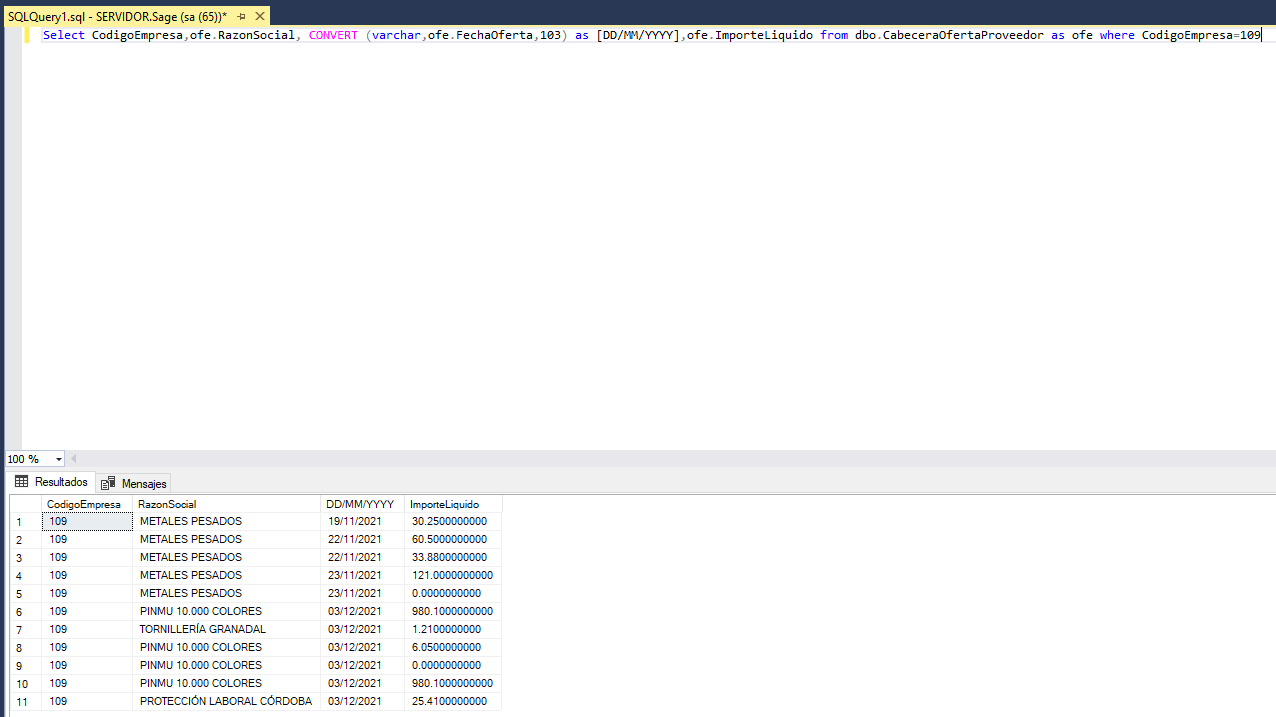
\includegraphics[scale = 0.45]{Consulta1.png}
        \caption{Primera consulta}
        \label{fig:my_label}
    \end{figure}
    
\newpage
  \section{Consulta 2}
    Capturas que muestren la consulta de las líneas de todos los albaranes de venta de tu empresa (utiliza el código de empresa) mostrando el código de la empresa, número de albarán, descripción del artículo y unidades.

    \begin{lstlisting}[style=C]
    SELECT al.CodigoEmpresa,al.NumeroAlbaran,
           al.DescripcionArticulo,al.Unidades 
    FROM dbo.LineasAlbaranCliente AS al 
    WHERE CodigoEmpresa=109
    \end{lstlisting}
    
    \begin{figure}[h]
        \centering
        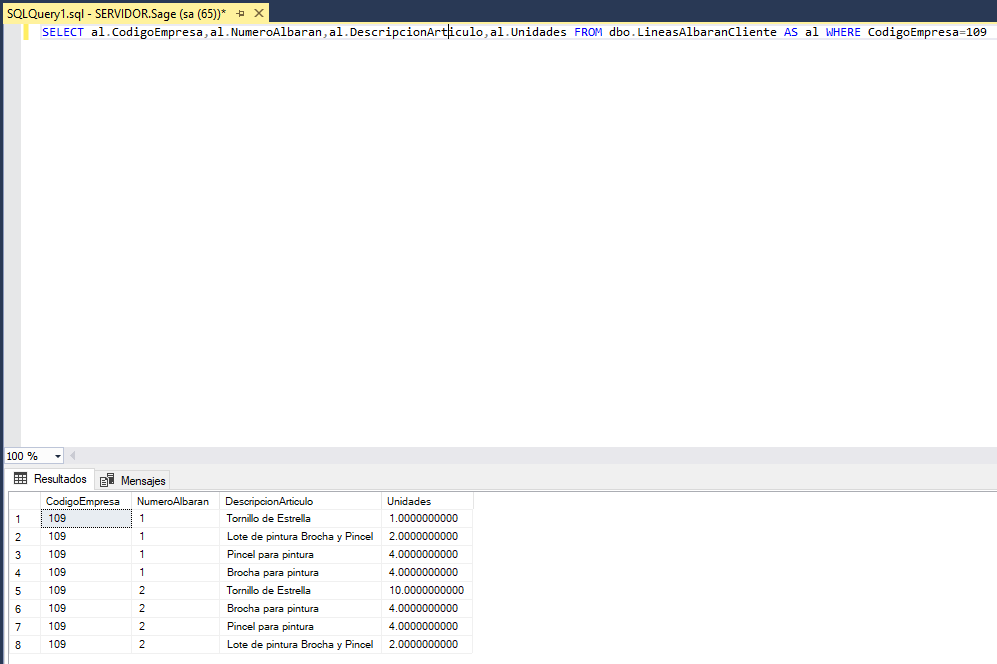
\includegraphics[scale = 0.5]{Consulta2.png}
        \caption{Segunda consulta}
        \label{fig:my_label}
    \end{figure}
    
\newpage
  \section{Consulta 3}
    Capturas que muestren la consulta de los pedidos de compra de un determinado proveedor mostrando todos los campos, pero utilizando una subconsulta en la que se obtenga el código del proveedor a partir de su nombre, por lo que no se pueden utilizar los campos "Razón social", "Nombre", etc de la tabla de pedidos de compra.

    \begin{lstlisting}[style=C]
    SELECT p.Nombre,lpp.*
    FROM dbo.LineasPedidoProveedor AS lpp, dbo.Empresas as em,
	     dbo.Proveedores as p
    WHERE p.Nombre='PCBOX' AND lpp.CodigodelProveedor = p.RazonSocial
    \end{lstlisting}
    
    \begin{figure}[h]
        \centering
        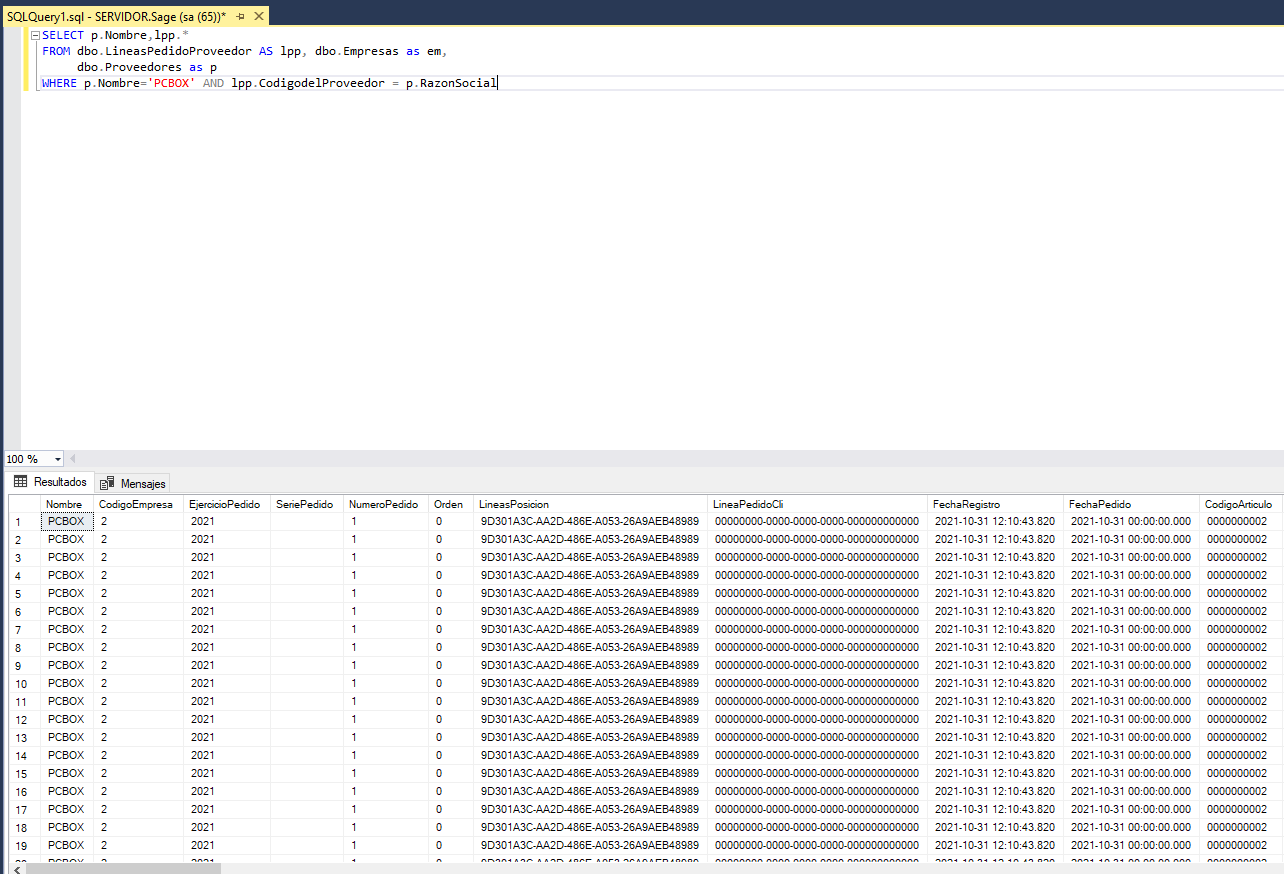
\includegraphics[scale = 0.45]{Consulta3.png}
        \caption{Primera consulta}
        \label{fig:my_label}
    \end{figure}
    
\newpage
  \section{Consulta 4}
    Capturas que muestren una consulta inventada por ti que relaciones dos tablas.

    \begin{lstlisting}[style=C]
    SELECT em.NombrePersona, al.CodigoEmpresa,
           al.NumeroAlbaran,al.DescripcionArticulo,
           al.Unidades 
    FROM dbo.LineasAlbaranCliente AS al, dbo.Empresas as em
    WHERE al.CodigoEmpresa=109 AND em.CodigoEmpresa = 109;
    \end{lstlisting}
    
    \begin{figure}[h]
        \centering
        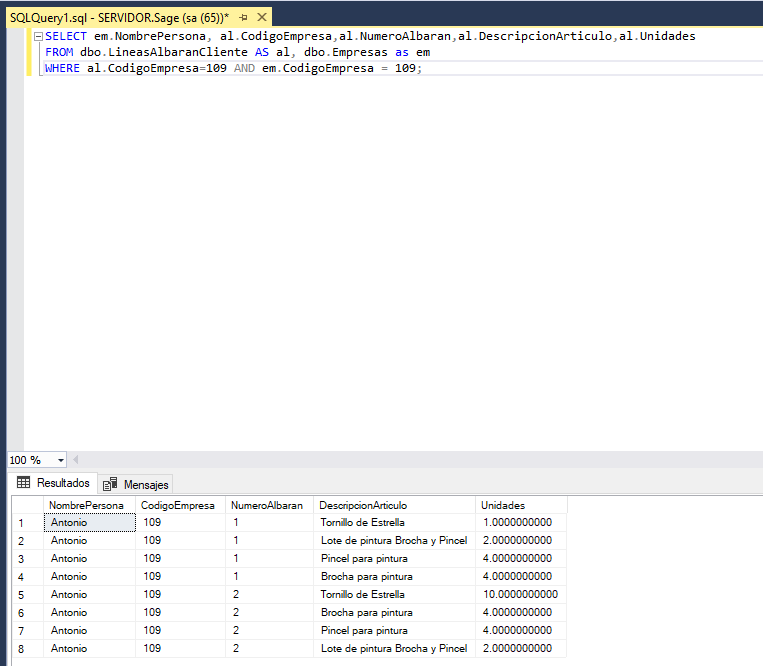
\includegraphics[scale = 0.45]{Consulta4.png}
        \caption{Primera consulta}
        \label{fig:my_label}
    \end{figure}

\end{document}